\nomenclature[F]{$n$}{Drehzahl \nomunit{$\frac{1}{\text{min}}$}}

\newvideofile{gleichstrommaschine1}{Gleichstrommaschine Teil 1}
\v{
	\begin{frame}{Lernziele}
		\begin{Lernziele}{Gleichstrommaschine}
			Du kannst
			\begin{itemize}
				\item das Prinzip eines Elektromotors erklären und welche Rolle die Lorentzkraft dabei spielt.
				\item die Hauptkomponenten einer Gleichstrommaschine benennen und deren Funktion beschreiben.
				\item die Berechnung der induzierten Spannung und des Drehmoments in einer Gleichstrommaschine durchführen.
				\item verschiedene Arten von Gleichstrommaschinen unterscheiden und ihre Anwendungsbereiche begründen.
			\end{itemize}
		\end{Lernziele}
		\speech{LernzieleGleichstrommaschine}{1}{In diesem Video Behandeln wir die Gleichstrommaschine. Dabei betrachten wir das Prinzip des Elektromotors und welche Rolle die Lorentz-kraft dabei spielt. Anschließend werfen wir einen Blick auf den Aufbau einer Gleichstrommaschine und werden Berechnungen dazu durchführen. Wir werden außerdem Drehmomentkennlienien betrachten und in diesem Zusammenhang die Anwendungsbereiche verschiedener Gleichstrommaschienen kennenlernen.}
		\silence{2}
	\end{frame}
}
\section{Gleichstrommaschine}
\s{
	Gleichstrommaschinen sind Elektromaschinen, die mit Gleichstrom betrieben werden und sowohl als Motoren als auch als Generatoren verwendet werden können. Sie zeichnen sich durch eine präzise Steuerbarkeit der Drehzahl und des Drehmoments aus, was sie ideal für Anwendungen mit variabler Geschwindigkeit und Last macht. Gleichstrommaschinen besitzen ein hohes Anlaufdrehmoment und ermöglichen eine einfache Umkehr der Drehrichtung. Sie werden häufig in Elektrofahrzeugen, industriellen Steuerungsanlagen und batteriebetriebenen Geräten eingesetzt.
}

\begin{frame}\ftx{Gleichstrommaschine Vorteile / Nachteile}
	\b{
		\f{}{height=0.5\textheight}{gleichstrommaschine1}{
		}{}
	}
	\pause
	\begin{minipage}{0.45\textwidth}
		\textbf{Vorteile:}
		\begin{itemize}
			\item Einfacher und kostengünstiger \\ Aufbau der Stromrichter
			\item Hohe Regeldynamik
			\item Direkter Betrieb der Maschine mit \\ Akkumulatoren möglich
			\item Große Überlastfähigkeit
		\end{itemize}
		\pause
	\end{minipage}\hfill
	\raisebox{3ex}{
		\begin{minipage}{0.45\textwidth}
			\textbf{Nachteile:}
			\begin{itemize}
				\item Hoher Konstruktionsaufwand
				\item Wartungsintensiv (Bürsten)
				\item Geringe Leistungsdichte
				\item Kosten
			\end{itemize}
		\end{minipage}
	}
	\speech{GleichstrommaschineVorNachteil}{1}{Gleichstrommaschinen sind elektrische Maschinen, die mit Gleichstrom betrieben werden und sowohl als Motoren als auch als Generatoren verwendet werden können. Sie zeichnen sich durch eine präzise Steuerbarkeit der Drehzahl und des Drehmoments aus, was sie ideal für Anwendungen mit variabler Geschwindigkeit und Last macht.}
	\speech{GleichstrommaschineVorNachteil}{2}{Ein Vorteil der Gleichstrommaschine ist der einfache Aufbau der Stromrichter, um die Drehzahl der Maschine einstellen zu können. Die Regeldynamik kann dabei sehr hoch sein, sodass sie gut unter variierenden Last-bedingungen eingesetzt werden können. Auch ist ein direkter Betrieb ohne jegliche Elektronik an Batterien möglich, was bei sehr einfachen Geräten wie zum Beispiel Spielzeugen ein großer Vorteil ist. Außerdem hat die Gleichstrommaschine eine hohe Überlastfähigkeit, was bedeutet, dass sie für eine bestimmte Zeit über ihre Nennlast hinaus belastet werden kann, ohne dass es zu Schäden oder einer nennenswerten Verringerung der Funktion kommt.}
	\silence{2}
	\speech{GleichstrommaschineVorNachteil}{3}{Ein wesentlicher Nachteil der Gleichstrommaschine ist der hohe Konstruktionsaufwand und die damit verbundenen höheren Kosten. Die notwendige Konstruktion mit Bürsten – auf die wir noch später in diesem Video eingehen werden – macht die Gleichstrommaschine wegen Abnutzung vergleichsweise wartungsintensiv. Außerdem ist die Leistungsdichte durch den Aufbau deutlich geringer als bei den anderen Maschinen-typen, was bedeutet, dass Gleichstrommaschinen im Verhältnis zu ihrer Leistung relativ groß ausfallen.}
	\silence{2}
\end{frame}

\begin{frame} \ftx{Elektrische Maschinen}
	\subsection{Exkurs Prinzip des Elektromotors\label{KapExkursLorentz}}
	\s{
		Zu Beginn werden die im Modul 6 vorgestellten Prinzipien aufgefrischt. Die Abbildung \ref{AbbLorentzSchleife} zeigt in drei Schaubildern kurzgefasst die Wirkungsweise eines Elektromotors. Zum grundlegenden Aufbau eines Elektromotors gehören ein feststehender Teil, Ständer\index{Ständer} oder Stator\index{Stator} genannt, und ein sich drehender Teil, auch Läufer\index{Läufer} oder Rotor\index{Rotor} genannt.
		In den drei Abbildungen ist eine Leiterspule in einem Hufeisenmagneten zu sehen. Der Hufeisenmagnet bildet hier den Stator, und eine um die eigene Achse bewegliche Leiterspule stellt den Rotor dar.
		Das erste Schaubild illustriert den isolierten Verlauf der magnetischen Feldlinien des Hufeisenmagneten. Sie verlaufen innerhalb des Hufeisenmagneten vertikal vom Nord- zum Südpol.
		Das zweite Schaubild zeigt den isolierten Verlauf der magnetischen Feldlinien der stromdurchflossenen Leiterschleife. Durch den Stromfluss entstehen an der Leiterschleife zwei entgegenwirkende Wirbelfelder.
		Im dritten Schaubild wird die Wechselwirkung des Hufeisenmagneten (Statorfeld) und der stromdurchflossenen Leiterschleife (Rotorfeld) aufgezeigt. Die beiden Felder überlagern sich. Die aus der Überlagerung resultierende Lorentzkraft bringt gemäß der Rechten‑Hand‑Regel die Leiterschleife zum Rotieren. Aus der elektromagnetischen Energie entsteht mechanische Energie.
	}
	\fu{
		\begin{minipage}{0.25\textwidth}
			\foo{width=0.9\textwidth, alt={Ein C-förmiger Permanentmagnet ist zu sehen, dessen Magnetfeld vom N-Pol zum S-Pol (von oben nach unten) verweist. Eine Leiterschleife, die sich innerhalb des Magnetfeldes befindet, ist transparent abgebildet und wird ignoriert, da sie nicht stromdurchflossen ist.}}{width=0.9\textwidth}{Lorentzkraft_Feldverlaeufe5}{
				\put(85, 78){\color{magnetfeld}N}
				\put(85, 15){\color{magnetfeld}S}
			}{}
		\end{minipage}
		\hfill
		\begin{minipage}{0.25\textwidth}
			\foo{width=0.9\textwidth, alt={Der C-förmige Permanentmagnet ist transparent abgebildet und wird nun ignoriert. Um die nun stromdurchflossene Leiterschleife entsteht ein magnetisches Feld in Abhängikeit der Flussrichtung.}}{width=0.9\textwidth}{Lorentzkraft_Feldverlaeufe6}{
				\put(5, 46.5){\color{magnetfeld}N}
				\put(55, 46.5){\color{magnetfeld}S}
				\put(-35, 47){\color{gray}+}
			}{}
		\end{minipage}
		\hfill
		\begin{minipage}{0.25\textwidth}
			\foo{width=0.9\textwidth, alt={Das Magnetfeld des C-förmigen Permanentmagneten und das Magnetfeld der stromdurchflossenen Leiterschleife werden zusammen betrachtet. Das Magnetfeld der Leiterschleife lenkt das Magnetfeld des Permanentmagneten in deren Zusammenspiel ab, sodass eine Kraft entsteht, die entgegen des Uhrzeigersinns wirkt. Dadurch dreht sich die Leiterschleife entsprechend gegen den Uhrzeigersinn.}}{width=0.9\textwidth}{Lorentzkraft_Feldverlaeufe7}{
				\put(85, 78){\color{magnetfeld}N}
				\put(85, 15){\color{magnetfeld}S}
				\put(8, 52){\color{gray}$F$}
				\put(54, 42){\color{gray}$F$}
				\put(-35, 47){\color{gray}$\Rightarrow$}
			}{}
		\end{minipage}
	}{{\bf Prinzip des Elektromotors.} Die Lorentzkraft bringt die sich im Magnetfeld befindende stromdurchflossene Leiterschleife in eine Drehbewegung. \label{AbbLorentzSchleife}}
	
	\s{Die Lorentzkraft kann mit der aus Modul 6 bekannten Formel berechnet werden:}
	\begin{eq}
		F =B\cdot I\cdot \ell\cdot N
	\end{eq}
	\speech{GleichstromPrinzipLorentzkraft}{1}{Um das im Modul 6 kennengelernte Prinzip des Elektromotors aufzufrischen, werfen wir nochmal einen Blick auf die Schaubilder zur Lorentz-kraft. In den drei Abbildungen ist eine Leiterspule innerhalb eines Hufeisenmagneten dargestellt. Das erste Schaubild illustriert den isolierten Verlauf der magnetischen Feldlinien des Hufeisenmagnets. Sie verlaufen innerhalb des Magneten wertikal von Nord- zum Südpol. Das zweite Schaubild zeigt den isolierten Verlauf der magnetischen Feldlinien der stromdurchflossenen Leiterschleife. Durch den Stromfluss entstehen an der Leiterschleife zwei entgegenwirkende Wirbelfelder. Im dritten Schaubild wird die Wechselwirkung des Hufeisenmagneten – dem Statorfeld – und der stromdurchflossenen Leiterschleife – dem Rotorfeld – aufgezeigt. Die beiden Felder überlagern sich. Die aus der Überlagerung resultierende Lorentzkraft bringt gemäß der Rechten-Hand-Regel die mittig drehbar gelagerte Leiterschleife zum rotieren. Aus der elektromagnetischen Energie entsteht also mechanische Energie.}
\end{frame}

\begin{frame} \ftx{Beispiel: Kraft einer Gleichstrommaschine}
	\begin{bsp}{Kraft einer Gleichstrommaschine}{}
		\onslide<2->{Ein Gleichstrommotor hat im Luftspalt eine magnetische Flussdichte von $B=0,8\,\mathrm{T}$. Unter den Polen befinden sich insgesamt $N=400$ Ankerdrähte, die mit einem Strom von $I=10\,\mathrm{A}$ durchflossen werden. Die wirksame Leiterlänge ist $\ell=150\,\mathrm{mm}$.}\\

		Berechnen Sie die Kraft $F$ am Umfang des Ankers.\pause
		\begin{align*}
			\onslide<3->{F & =B\cdot I\cdot \ell\cdot N }                                                                                                                            \\
			\onslide<4->{  & =0,8\,\frac{\mathrm{Vs}}{\mathrm{m}^2}\cdot 10\,\mathrm{A}\cdot0,15\,\mathrm{m}\cdot 400}                                                               \\
			\onslide<5->{  & =480\,\frac{\mathrm{kg}\cdot\mathrm{m}^2\cdot\mathrm{s}\cdot\mathrm{A}\cdot\mathrm{m}}{\mathrm{s}^3\cdot\mathrm{A}\cdot\mathrm{m}^2} = 480\,\mathrm{N}}
		\end{align*}

	\end{bsp}
	\speech{GleichstrommaschinePrinzip}{1}{Kommen wir als kurze Wiederholung zu einem Beispiel zur Berechnung der Kraft einer Gleichstrommaschine. Die grundlegenden Prinzipien, die hinter der Funktion einer Gleichstrommaschine stecken, wurden im Modul sechs bereits vorgestellt. Sie basiert auf der Lorentz-Kraft. Ebenso kennen wir bereits die Formel zur Berechnung der Lorentz-Kraft.}
	\silence{2}
	\speech{GleichstrommaschinePrinzip}{2}{Gegeben ist ein Gleichstrommotor mit einer Flussdichte B von 0,8 Tesla im Luftspalt. Die Ankerdrähte der Pole haben 400 Windungen und werden mit 10 Ampere durchflossen. Die Leiterlänge L innerhalb des Magnetfelds ist Hundertfünfzig Millimeter. Hierzu soll nun die Kraft F am Anker berechnet werden.}
	\silence{2}
	\speech{GleichstrommaschinePrinzip}{3}{Die Formel zur Berechnung der Lorentz-Kraft kennen wir ja schon. Außerdem sind alle notwendigen Größen in dem Beispiel gegeben.}
	\speech{GleichstrommaschinePrinzip}{4}{Wir müssen also nur die Werte in die Formel einsetzen. Dabei schreiben wir zum leichteren Kürzen der Einheiten die Einheit Tesla direkt als Volt-Sekunden pro Meter zum Quadrat.}
	\speech{GleichstrommaschinePrinzip}{5}{Nun berechnen wir die Werte und kürzen anschließend die Einheiten. Es verbleiben gekürzt Vierhundertachzig Kilogramm mal Meter, geteilt durch Sekunden zum Quadrat. Das entspricht Vierhundertachzig Newton.}
	\silence{2}
\end{frame}

\s{
	\subsection{Aufbau und Gehäusekonstruktion}\index{Gleichstrommaschine>Aufbau}
}
\begin{frame}\ftx{Aufbau}
	\s{
		Der Aufbau der Gleichstrommaschine wird anhand dreier Abbildungen dargestellt. Abbildung \ref{GrafikGleichstrommaschine} zeigt ein diagonales Schnittmodell der Gleichstrommaschine, das eine allgemeine Übersicht über die Komponenten von Stator und Rotor gibt. Zur detaillierteren Veranschaulichung des Aufbaus werden die Abbildung \ref{QuerschnittGleichstrommaschine} mit Fokus auf dem Stator und Abbildung \ref{FotoRotor} zur Veranschaulichung des Rotors einer Gleichstrommaschine herangezogen.

		\nomenclature[F]{$p$}{Polpaarzahl}
	}
	\fo{width=0.6\textwidth, alt={Das Bild zeigt einen Einblick in eine Gleichstrommaschine. Im Zentrum des Bildes befindet sich der Rotorzylinder, der auf einer Welle befestigt ist, welche durch Kugellager frei drehbar am Motorgehäuse gelagert ist. Um den Rotorzylinder sind die Wicklungen des Rotors angeordnet, die in ihrer charakteristischen Spulenform dargestellt sind. Am linken Ende der Welle sind die Kommutatorlamellen erkennbar, die ringförmig um die Welle angeordnet sind. Elektrische Leiter führen von den Kommutatorlamellen zu den Spulenwicklungen des Rotors. Die Spulen verlaufen innerhalb des Rotorzylinders. Am Gehäuse befestigt befinden sich um den Rotorzylinder herum Erregerpole mit Wicklungen.}}{height=0.85\textheight}{gleichstrommaschine1}{
		\put(70,0){\line(-1,1){38}}\put(70.3,0){Kommutatorlamellen}
		\put(86,8){\line(-1,1){56}}\put(86.3,8){Erregerpole mit Wicklung}
		\put(90,16){\line(-1,1){45}}\put(90,16){Wicklungen des Rotors}
		\put(95,24){\line(-1,1){28}}\put(95.3,24){Rotorzylinder}
		\put(105,32){\line(-1,1){28}}\put(105.3,32){Lager}
	}{{\bf Grafik einer aufgeschnittenen Gleichstrommaschine.}  \label{GrafikGleichstrommaschine}}

	\speech{GleichstrommaschineAufbau1}{1}{Eine Gleichstrommaschine besteht aus mehreren Komponenten, die gemeinsam für die Umwandlung von elektrischer Energie in mechanische Energie und umgekehrt verantwortlich sind. Im Zentrum steht der Rotorzylinder, der drehbar gelagert und mit Wicklungen ausgestattet ist. Diese Wicklungen sind Drahtwindungen, die ein Magnetfeld erzeugen, wenn elektrischer Strom hindurchfließt. Um den Rotor herum befinden sich die Erregerpole, die ein externes Magnetfeld bereitstellen. Die Lager sind entscheidend für die Stabilität, da sie den Rotor in Position halten und eine reibungslose Drehung ermöglichen. Ein weiteres zentrales Element einer Gleichstrommaschine ist der Kommutator, der aus einzelnen Lamellen besteht. Der Kommutator ist ein mechanischer Schalter und sorgt dafür, dass der Strom während der Drehung des Rotors regelmäßig in den Wicklungen umgekehrt wird. Das ist notwendig, um eine gleichbleibende Drehbewegung des Rotors zu gewährleisten.}
	\silence{2}
\end{frame}


\begin{frame}\ftx{Aufbau}

	\s{
		\fo{width=0.8\textwidth, alt={Das Bild zeigt den Querschnitt einer Gleichstrommaschine mit zwei Polen, die detailliert die inneren Komponenten zeigt. In der Mitte der kreisförmigen Anordnung befindet sich an einer Achse der Rotorzylinder, an dessen äußeren Rand die Wicklungen verlaufen. Um den Rotorzylinder bedinden sich halbkreisförmig oben und unten die beiden Pole mit den Kompensationswicklungen. Zwischen Rotorzylinder und den Polen befindet sich ein schmaler Luftspalt. Die Pole sind jeweils über einen Polschuh mit dem ringförmigen Ständerjoch verbunden, das die gesamte Anordnung umgibt. Innerhalb des Ständerjochs befinden sich jeweils auf der linken und rechten Seite Wendepole mit Wicklungen.}}{}{Aufbau1}{
			\put(27,20){\line(1,1){16}}\put(-5,20){Wendepole mit Wicklung}
			\put(30.5,15){\line(1,1){22}}\put(-5,15){Rotorzylinder mit Wicklung}
			\put(40,5){\line(1,1){17}}\put(9.5,5){Kompensations\-wicklung}
			\put(40.5,0){\line(1,1){14}}\put(9.5,0){Pol mit Erregerwicklung}
			\put(85,5){\line(-1,1){14}}\put(85.3, 5){Polschuh}
			\put(85,0){\line(-1,1){8}}\put(85.3,0){Ständerjoch}
		}{{\bf Grundlegender Aufbau einer Gleichstrommaschine.} Hier mit nur einem Polpaar (Polpaarzahl $p=1$). \label{QuerschnittGleichstrommaschine}}
		Die Komponenten des Stators, auch Ständer genannt, werden im frontalen Querschnitt einer Gleichstrommaschine (Abbildung \ref{QuerschnittGleichstrommaschine}) gut veranschaulicht. Eine der grundlegenden Komponenten ist die Erregerwicklung\index{Erregerwicklung}, die um einen Polschuh gewunden, einen Pol darstellt. Die Pole haben die Aufgabe, ein Magnetfeld, Erregerfeld genannt, zu erzeugen.

		Da ein magnetisches Feld immer einen Nord- und einen Südpol beinhaltet, werden die Pole paarweise gegenüber eingebaut. Die daraus resultierende Kenngröße, die Polpaarzahl, gibt Aufschluss über die Betriebseigenschaften der Gleichstrommaschine.
		Eine höhere Polpaarzahl verringert die Drehzahl, erhöht jedoch das Drehmoment. Bei Kleinstmaschinen können die Erregerwicklungen durch Permanentmagnete ersetzt werden.
		Bei größeren Maschinen (ca. über 1 kW) sind zusätzlich Wendepolwicklungen vorhanden.
	}
	\b{
		\fo{}{height=0.85\textheight}{Aufbau1}{
			\put(27,20){\line(1,1){16}}\put(-9,20){Wendepole mit Wicklung}
			\put(30.5,15){\line(1,1){22}}\put(-9,15){Rotorzylinder mit Wicklung}
			\put(40,5){\line(1,1){17}}\put(5.5,5){Kompensations\-wicklung}
			\put(40.5,0){\line(1,1){14}}\put(5.5,0){Pol mit Erregerwicklung}
			\put(85,5){\line(-1,1){14}}\put(85.3, 5){Polschuh}
			\put(85,0){\line(-1,1){8}}\put(85.3,0){Ständerjoch}
		}{}
	}

	\speech{GleichstrommaschineAufbau2}{1}{Die Komponenten des Sta-tors, der auch Ständer genannt wird, sind im frontalen Querschnitt gut zu sehen. Eine der grundlegenden Komponenten ist die Erregerwicklung. Sie ist um einen Pohlschuh gewunden. Erregerwicklung und Pohlschuh stellen zusammen einen Pohl dar. Die Pole haben die Aufgabe, ein Magnetfeld, auch Erregerfeld genannt, zu erzeugen. Da ein magnetisches Feld immer einen Nord- und einen Südpol beinhaltet, werden die Pole paarweise gegenüberliegend eingebaut. Die sich daraus ergebende Kenngröße ist die Polpaarzahl. Sie gibt Aufschluss über die Betriebseigenschaften der Gleichstrommaschine. Eine höhere Pohlpaarzahl verringert die Drehzahl, erhöht jedoch das Drehmoment. Bei Kleinstmaschinen können die Erregerwicklungen durch Permanentmagnete ersetzt werden. Bei größeren Maschinen, ab ungefähr ein Kilowatt Leistung, sind zusätzlich Wendepolwicklungen vorhanden.}
	\silence{2}
\end{frame}

\begin{frame} \ftx{Rotor und Kommutator}
	\s{
		In der Abbildung \ref{FotoRotor} sind die Komponenten des Rotors gut ersichtlich. Im Allgemeinen wird der Rotor auch Anker oder als Läufer bezeichnet. Die Funktion des Rotors besteht darin, die elektromagnetische Energie durch Rotationen um die eigene Achse in mechanische Energie (und umgekehrt) zu wandeln.
		Hierzu ist der Rotor an einer Motorwelle befestigt, die die mechanische Energie überträgt. Das Kugellager am Ende der Motorwelle verringert dabei die Reibungsverluste bei der Energieübertragung.
		Um den Rotor in Bewegung zu bringen, ist das Zusammenwirken von Kommutator und Rotorwicklung wichtig. Die Rotorwicklung, auch Ankerwicklung bezeichnet, hat die Aufgabe ein magnetisches Feld, das Ankerfeld, zu erzeugen. Erst durch die Interaktion des Ankerfelds mit dem Erregerfeld wird ein Drehmoment auf den Rotor ausgeübt und setzt diesen in Bewegung.
		Die Blechwände, um die die Spulen gewickelt sind, bestehen aus isolierenden Blechen, um Wirbelströme in den Wicklungen zu reduzieren.
		Der Kommutator\index{Kommutator} oder Stromwender\index{Stromwender} hat die Funktion, die Rotorwicklung getaktet mit Strom zu versorgen. Er besteht aus mehreren voneinander getrennten Lamellen, die jeweils mit einem Strang der Rotorwicklung verbunden sind.
		Der Strom wird nun über am Stator angebrachten Kohlebürsten an die Kommutatorlamellen geleitet. Durch die Drehung der Lamellen unter den Bürsten wirkt der Kommutator als mechanischer Schalter und sorgt dafür, dass die Stromrichtung in den Rotorwicklungen, die sich jeweils unter den Hauptpolen befinden, gleich bleibt.
	}
	\fo{width=0.8\textwidth, alt={Fotografie eines Rotors ohne Gehäuse. Am vorderen Ende des Rotors befindet sich ein Lager, gefolgt vom Kommutator. Dahinter sind die Wicklungen sichtbar, die durch das weiter hinten liegende Blechpoaket des Rotors führen.}}{width=0.75\textwidth}{Rotor_Gleichstrommaschine_kl}{
		\put(87,45){\line(-1,1){10}}\put(87,45){Welle}
		\put(65,20){\line(-1,1){10}}\put(65.3,20){Blechpaket}
		\put(48,10){\line(-1,1){10}}\put(48,10){Wicklungen}
		\put(35,5){\line(-1,1){10}}\put(35.3,5){Kommutator}
		\put(23,0){\line(-1,1){10}}\put(23.3,0){Lager}
	}{{\bf Foto eines Rotors.} Zu erkennen sind hier die charakteristischen Bauelemente. \index{Gleichstrommaschine>Rotor}\label{FotoRotor}}

	\speech{GleichstrommaschineAufbau3}{1}{Hier sehen wir einen Rotor einer Gleichstrommaschine. Der Rotor wird auch als Anker oder Läufer bezeichnet. Die Funktion des Rotors besteht darin, die elektromagnetische Energie durch Rotationen um die eigene Achse in mechanische Energie und umgekehrt zu wandeln. Hierzu ist der Rotor an einer Motorwelle befestigt, die die mechanische Energie überträgt. Das Kugellager am Ende der Motorwelle verringert dabei die Reibungsverluste bei der Energieübertragung. Um den Rotor in Bewegung zu bringen, ist das Zusammenwirken von Kommutator und Rotorwicklung wichtig. Die Rotorwicklung, die auch Ankerwicklung genannt wird, hat die Aufgabe ein magnetisches Feld, das Ankerfeld, zu erzeugen. Erst durch die Interaktion des Ankerfelds mit dem Erregerfeld wird ein Drehmoment auf den Rotor ausgeübt und setzt diesen in Bewegung. Die Blechwände, um die die Spulen gewickelt sind, bestehen aus isolierenden Blechen, um Wirbelströme in den Wicklungen zu reduzieren. Der Kommutator, der auch Stromwender genannt wird, hat die Funktion, die Rotorwicklung getaktet mit Strom zu versorgen. Er besteht aus mehreren voneinander getrennten Lamellen, die jeweils mit einem Strang der Rotorwicklung verbunden sind. Der Strom wird nun über am Stator angebrachten Kohlebürsten an die Kommutatorlamellen geleitet. Durch die Drehung der Lamellen unter den Bürsten wirkt der Kommutator als mechanischer Schalter und sorgt dafür, dass die Stromrichtung in den Rotorwicklungen gleich bleibt.}
	\silence{2}
\end{frame}

\s{\subsection{Magnetische Felder}\index{Gleichstrommaschine>Felder}}
\begin{frame}\ftx{Erregerfeld}
	\s{Für die Lorentzkraft ist das magnetische Feld entscheidend, in dem sich der Leiter bewegt. Dieses Feld wird durch den Stator mit den Erregerwicklungen erzeugt und ist im Bereich des Rotors näherungsweise parallel und homogen.
	}
	\fo{width=0.6\textwidth, alt={Eine schematische Grafik, die den Querschnitt einer Gleichstrommaschine zeigt. In der ringförmigen Anordnung sind die Magnetfelder durch Magnetfeldlinien eingezeichnet. Diese verlaufen geschwungen vom N-Pol (oben) zum S-Pol (unten) innerhalb der Polschuhe. Dabei nutzen sie das Volumen des Materials aus. An der Stelle, an der das Magnetfeld  den Luftspalt zum Rotorzylinder überwindet, verlaufen die Magnetfeldlinien auf dem kürzesten Weg gerade in den Rotorzylinder. Innerhalb des Rotorzylinders nutzen die Magnetfeldlinien wieder das Volumen des Material bestmöglich aus, bis sie auf der unteren Seite wieder den Luftspalt zum zweiten Polschuh auf der kürzesten Strecke überwinden. Die Magnetfeldlinien schließen sich innderhalb des Ständerjochs, das die Anordnung umschließt und fließen im Ständerjoch vom S-Pol um N-Pol zurück.}}{height=0.85\textheight}{Erregerfeld}{
		\put(50,97){\color{magnetfeld}\makebox[0pt]{N}}
		\put(50,0){\color{magnetfeld}\makebox[0pt]{S}}
	}{{\bf Erregerfeld einer Gleichstrommaschine.} Schematische Darstellung in der Vorderansicht.}

	\speech{GleichstrommaschineErregerfeld}{1}{In dieser schematischen Darstellung des Querschnitts durch eine Gleichstrommaschine werden in orange die Feldlinienverläufe des Erregerfeldes dargestellt. Für die Lorentz-Kraft ist das magnetische Feld, in dem sich der Leiter bewegt, entscheidend. Dieses Feld wird durch den Stat-or mit den Erregerwicklungen erzeugt und ist im Bereich des Rotors näherungsweise parallel und homogen. Das Drehmoment einer Gleichstrommaschine ist direkt proportional zur Lorentz-Kraft, die durch das Erregerfeld erzeugt wird. Je stärker und homogener das magnetische Feld im Rotor ist, desto größer ist das erzeugte Drehmoment.}
	\silence{2}
\end{frame}

\newvideofile{gleichstrommaschine2}{Gleichstrommaschine Teil 2}
\begin{frame}\ftx{Induzierte Spannung}
	\s{\subsection{Berechnung des Drehmoments}}
	\s{
		In Modul 6 und Kapitel \ref{KapExkursLorentz} ist bereits die Kraftwirkung auf einen stromdurchflossenen Leiter im Magnetfeld erklärt worden. Um das Drehmoment der Gleichstrommaschine zu berechnen, wird zuerst die induzierte Spannung ermittelt (siehe Modul 6). Dreht sich der Rotor einer erregten Gleichstrommaschine, wird in jeder Leiterschleife des Ankers eine Spannung induziert. Nach dem Induktionsgesetz (Gleichung \ref{GlInduktionsgesetz}) ist die Höhe der induzierten Spannung (Quellenspannung) $U_\mathrm{q}$ vom magnetischen Fluss $\varPhi$ und der zeitlichen Änderung, in diesem Fall der Drehzahl $n$ bzw. der damit verknüpften Kreisfrequenz $\omega = 2\pi\cdot n$ abhängig.
		Werden hierzu noch die spezifischen geometrischen Gegebenheiten des Rotors in Form der Ankerkonstanten $K$ multipliziert, so ergibt das Produkt aus diesen Kenngrößen die induzierte Spannung $U_\mathrm{q}$ der Gleichstrommaschine (siehe Gleichung \ref{GlInduzierteSpannungGM}).
	}

	\begin{eq}
		\onslide<7->{U_\mathrm{q} = K \cdot \varPhi \cdot \omega \label{GlInduzierteSpannungGM}}
	\end{eq}
	\b{
		\begin{itemize}
			\onslide<2->{\item Induzierte Spannung (Quellenspannung): $U_\mathrm{q}$ [V]}
			      \onslide<6->{\item Ankerkonstante: $K$ [1]\index{Ankerkonstante} \nomenclature[F]{$K$}{Ankerkonstante der Gleichstrommaschine}}
			      \onslide<3->{\item Fluss: $\varPhi$ [Vs]}
			      \onslide<4->{\item Drehzahl $n$} \onslide<5->{$\Rightarrow$ Winkelgeschwindigkeit: $\omega_\mathrm{mech}$ ($= 2\pi\cdot n$) [rad/s]}
		\end{itemize}
	}	\pause

	\s{
		Wenn sowohl die elektrischen als auch mechanischen Verluste vernachlässigt werden, kann die induzierte Spannung kann auch direkt über die sogenannte innere Leistung $P_\mathrm{i}$ angegeben werden. Diese entspricht dann sowohl der elektrischen Leistung $U_\mathrm{q}\cdot I_\mathrm{A}$, als auch der mechanischen Leistung $P_\mathrm{mech}$, welche sich aus dem Produkt des inneren Drehmoments $M_\mathrm{i}$ und der Winkelgeschwindigkeit $\omega$ errechnet.
	}
	\begin{eq}
		\onslide<9->{P_\mathrm{i} = U_\mathrm{q}\cdot I_\mathrm{A} =  P_\mathrm{mech} = M_\mathrm{i}\cdot \omega \label{GlGMWirkungsgrad}}
	\end{eq}

	\b{
		\begin{itemize}
			\onslide<8->{\item innere elektrische Leistung: $P_\mathrm{i}$ [W]}
		\end{itemize}
	}
	\speech{GleichstomDrehmomentberechnung}{1}{Nachdem wir im vorangegangenen Video den Aufbau einer Gleichstrommaschine kennengelernt haben, schauen wir uns nun an, wie das Drehmoment einer Gleichstrommaschine berechnet wird. In Modul 6 wurde bereits die Kraftwirkung auf einen stromdurchflossenen Leiter im Magnetfeld thematisiert. Um das Drehmoment der Gleichstrommaschine zu berechnen, wird zuerst die induzierte Spannung ermittelt.}
	\silence{2}
	\speech{GleichstomDrehmomentberechnung}{2}{Dreht sich der Rotor einer erregten Gleichstrommaschine, wird in jeder Leiterschleife des Ankers eine Spannung induziert.}
	\silence{2}
	\speech{GleichstomDrehmomentberechnung}{3}{Nach dem Induktionsgesetz ist die Höhe der induzierten Spannung U-Q, auch Quellenspannung genannt, vom magnetischen Fluss Phi abhängig.}
	\speech{GleichstomDrehmomentberechnung}{4}{Aber ebenso von der zeitlichen Änderung. In diesem Fall ist das die Drehzahl klein N.}
	\speech{GleichstomDrehmomentberechnung}{5}{Beziehungsweise die damit verknüpfte Kreisfrequenz Omega. Diese Kreisfrequenz entspricht 2 Pi mal der Drehzahl klein N.}
	\silence{2}
	\speech{GleichstomDrehmomentberechnung}{6}{Nun werden hierzu noch die spezifischen geometrischen Gegebenheiten des Rotors in Form der Ankerkonstanten K multipliziert.}
	\speech{GleichstomDrehmomentberechnung}{7}{So ergibt das Produkt aus diesen Kenngrößen die induzierte Spannung U-q der Gleichstrommaschine.}
	\silence{2}
	\speech{GleichstomDrehmomentberechnung}{8}{Wenn sowohl die elektrischen als auch mechanischen Verluste vernachlässigt werden, kann die induzierte Spannung auch direkt über die sogenannte innere Leistung P-I angegeben werden.}
	\silence{2}
	\speech{GleichstomDrehmomentberechnung}{9}{Diese entspricht dann sowohl der elektrischen Leistung U-Q mal I-A, als auch der mechanischen Leistung P-Mech, welche sich aus dem Produkt des inneren Drehmoments M-I und der Winkelgeschwindigkeit Omega errechnet.}
	\silence{2}
\end{frame}

\begin{frame}\ftx{Inneres Moment}
	\s{Wird diese Erkenntnis nun in Gleichung \ref{GlInduzierteSpannungGM} eingesetzt, errechnet sich das innere Drehmoment $M_\mathrm{i}$ aus dem Produkt der Ankerkonstante $K$, dem magnetischen Fluss $\varPhi$ und dem Ankerstrom $I_\mathrm{A}$}
	\begin{eq}
		M_\mathrm{i} = K \cdot \varPhi \cdot I_\mathrm{A} \label{GlMomentGM}
	\end{eq}
	\b{
		\begin{itemize}
			\item Inneres elektrisches Moment:  $M_\mathrm{i}$ [Nm]
			\item Ankerkonstante: $K$ [1]
			\item Fluss: $\varPhi$ [Vs]
			\item Ankerstrom: $I_\mathrm{A}$  [A]
		\end{itemize}\pause
	}
	\s{
		Im Motorbetrieb ist das Drehmoment an der Welle der Maschine das innere Drehmoment $M_\mathrm{i}$ abzüg\-lich der Verluste $M_\mathrm{V}$. Das Maschinenmoment kann auch durch den Wirkungsgrad $\eta_1$ ausgedrückt werden. Dieser Wirkungsgrad vernachlässigt allerdings die elektrischen Verluste durch den Ankerwiderstand und der Erregung.
	}
	\begin{eq}
		M = M_\mathrm{i} - M_\mathrm{V}\qquad \qquad M = \eta_1\cdot M_\mathrm{i}\label{GLMomentWirkungsgradGM}
	\end{eq}
	\begin{itemize}
		\item Verlustmoment: $M_\mathrm{V}$ [Nm]
		\item Wirkungsgrad:  $\eta$ [1]
	\end{itemize}

	\speech{GleichstomInneresDrehmoment}{1}{Wird diese Erkenntnis nun in die vorangegangene Gleichung eingesetzt, errechnet sich das innere Drehmoment M-I aus dem Produkt der Ankerkonstanten K, dem magnetischen Fluss Fie und dem Ankerstrom Ih-A.}
	\silence{2}
	\speech{GleichstomInneresDrehmoment}{2}{Im Motorbetrieb ist das Drehmoment an der Welle der Maschine das innere Drehmoment M-I abzüglich der Verluste M-V. Das Maschinenmoment kann auch mit dem Wirkungsgrad Eta Eins ausgedrückt werden. Dieser Wirkungsgrad vernachlässigt allerdings die elektrischen Verluste durch den Ankerwiderstand und der Erregung.}
	\silence{2}
\end{frame}

\s{\subsection{Fremderregte Gleichstrommaschine}}
\begin{frame}\ftx{Fremderregte Gleichstrommaschine}
	\s{Der Erregerkreis im Stator der Gleichstrommaschine und der Rotorkreis, der über den Kommutator mit Strom versorgt wird, sind prinzipiell unabhängig voneinander. Wenn beide Stromkreise von unterschiedlichen Spannungsquellen versorgt werden, wird die Maschine fremderregt genannt. \index{Gleichstrommaschine>Fremderregt} Das Ersatzschaltbild ist in Abbildung \ref{AbbGMFremderregt} dargestellt.}
	\fu{
		\input{Tikz/src/ersatzschaltbild_fremderegte_Gleichstromm}\alttext{Schaltbild einer fremderregten Gleichstrommaschine, bestehend aus zwei Teilen: Im Erregerkreis, links, befindet sich ein Widerstand (RE) und eine Induktivität (LE), die über eine Spannungsquelle (UE) verbunden sind. Im Ankerkreis, rechts, befindet sich ein Widerstand (RA) und ein mit "GM" bezeichnetet Bauteil, das für eine Induktivität, als auch Spannungsquelle steht. Der Widerstand (RA) und das Bauteil "GM" sind über eine Spanungsquelle (UA) verbunden.}
	}{{\bf Ersatzschaltbild einer fremderregten Gleichstrommaschine.} \label{AbbGMFremderregt}}
	\s{Der Erregerkreis besteht aus der Induktivität der Erregerwicklung $L_\mathrm{E}$ und dem Kupferwiderstand $R_\mathrm{E}$ der Spule. Im Ankerkreis wird die Wicklung als Kreis mit angedeuteten Schleifringen dargestellt, da sie einerseits eine Induktivität, als auch eine Spannungsquelle darstellt. Auch der Anker hat einen ohmschen Widerstand $R_\mathrm{A}$.

		Der Maschenumlauf im Rotorkreis ergibt:}
	\begin{eq}
		U_\mathrm{A} = U_\mathrm{q} + I_\mathrm{A}\cdot R_\mathrm{A}
	\end{eq}

	\s{Durch Einsetzen von Gleichung \ref{GlInduzierteSpannungGM} und \ref{GlMomentGM} ergibt sich die Drehzahl/Drehmoment- und Ankerstromkennlinie für die fremderregte Gleichstrommaschine:}
	\s{
		\begin{eq}
			n = \frac{U_\mathrm{A}}{2\pi K\cdot \varPhi} - \frac{R_\mathrm{A}\cdot M_\mathrm{i}}{2\pi(K\cdot \varPhi)^2}\label{GlfremderregteGM1}
		\end{eq}
	}
	\b{
		\begin{eq}
			n = \frac{U_\mathrm{A}}{2\pi K\cdot \varPhi} - \frac{R_\mathrm{A}\cdot M_\mathrm{i}}{2\pi(K\cdot \varPhi)^2}
			\qquad \qquad I_\mathrm{A} = \frac{M_\mathrm{i}}{K\cdot \varPhi}
		\end{eq}
	}

	\speech{FremderregteGleichstommaschine}{1}{Bei der fremderregten Gleichstrommaschine sind der Erregerkreis im Stator und der Rotorkreis, der über den Kommutator mit Strom versorgt wird, prinzipiell unabhängig voneinander. Wenn beide Stromkreise von unterschiedlichen Spannungsquellen versorgt werden, wird die Maschine fremderregt genannt. Das Ersatzschaltbild einer solchen fremderregten Gleichstrommaschine ist hier gezeigt. Der Erregerkreis besteht aus der Induktivität der Erregerwicklung L-E und dem Kupferwiderstand R-E der Spule. Im Ankerkreis wird die Wicklung als Kreis mit angedeuteten Schleifringen dargestellt, da sie einerseits eine Induktivität, als auch eine Spannungsquelle darstellt. Auch der Anker hat einen ohmschen Widerstand R-A.}
	\silence{2}
	\speech{FremderregteGleichstommaschine}{2}{Der Maschenumlauf im Rotorkreis ergibt: Die Anker-Spannung U-A ist gleich der Summe aus Spannung U-Q und dem Produkt aus dem Anker-Strom Ih-A und dem Anker-Widerstand R-A.}
	\silence{2}
	\speech{FremderregteGleichstommaschine}{3}{Durch Einsetzen von der Gleichung zur Berechnung der Anker-Spannung U-A und der Gleichung zur Berechnung des Drehmoment M-I, die wir beide zuvor schon kennengelernt haben, ergibt sich nach Umstellung der neuen Gleichung die Drehzahl-Drehmoment- und Ankerstromkennlinie für die fremderregte Gleichstrommaschine.}
	\silence{2}
\end{frame}


\begin{frame}\ftx{Beispiel: Fremderregte Gleichstrommaschine}
	\s{
		\begin{bsp}{Fremderregte Gleichstrommaschine}{}
			Eine fremderregte Gleichstrommaschine mit der Ankerkonstante $K=\frac{1}{2\pi}$ hat bei der Spannung $U_\mathrm{A}=400\,\text{V}$ eine Leerlaufdrehzahl von $n=1200\,\frac{1}{\text{min}}$. Der Ankerwiderstand beträgt $R_\mathrm{A}=2,3\,\Omega$.
			\begin{itemize}
				\item [a)] Wie groß ist der Erregerfluss $\varPhi$?

				      Im Leerlauf ist das innere Drehmoment $M_\mathrm{i}$ gleich Null. Gleichung \ref{GlfremderregteGM1} vereinfacht sich daher zu:
				      \begin{align*}
					      n       & =\frac{U_\mathrm{A}}{2\pi K\cdot \varPhi}                                                                                                                                      \\
					      \varPhi & =\frac{U_\mathrm{A}}{2\pi K\cdot n} = \frac{400\,\text{V}}{\frac{2\pi}{2\pi}\cdot 1200 \,\frac{1}{\text{min}}\cdot \frac{1}{60\,\frac{\text{s}}{\text{min}}}}  = 20\,\text{Vs}
				      \end{align*}

				\item[b)] Wie schnell dreht die Maschine bei einem inneren Drehmoment von $M_\mathrm{i}=10\,\text{Nm}$?
				      \begin{align*}
					      n & = \frac{U_\mathrm{A}}{2\pi K\cdot \varPhi} - \frac{R_\mathrm{A}\cdot M_\mathrm{i}}{2\pi(K\cdot \varPhi)^2}                                       \\
					        & = \frac{400\,\text{V}}{\frac{2\pi}{2\pi}\cdot 20\,\text{Vs}} - \frac{2,3\,\Omega \cdot 10\,\text{Nm}}{2\pi(\frac{1}{2\pi}\cdot 20\,\text{Vs})^2} \\
					        & = 20\,\frac{1}{\text{s}} - 0,362 \,\frac{1}{\text{s}} = 19,638\,\frac{1}{\text{s}} =  1178,3\,\frac{1}{\text{min}}
				      \end{align*}
				\item[c)] Wie groß ist der Ankerstrom?
				      \begin{align*}
					      I_\mathrm{A} & = \frac{M_\mathrm{i}}{K\cdot \varPhi} = \frac{10\,\text{Nm}}{\,\frac{1}{2\pi}\cdot 20\,\text{Vs}\,} = 3,61\,\text{A}
				      \end{align*}
			\end{itemize}
		\end{bsp}
	}
	\b{
		Eine fremderregte Gleichstrommaschine mit der Ankerkonstante $K=\frac{1}{2\pi}$ hat bei der Spannung $U_\mathrm{A}=400\,\text{V}$ eine Leerlaufdrehzahl von $n=1200\,\frac{1}{\text{min}}$. Der Ankerwiderstand beträgt $R_\mathrm{A}=2,3\,\Omega$.
		\begin{itemize}
			\item [a)] Wie groß ist der Erregerfluss $\varPhi$? \pause

			      Im Leerlauf ist das innere Drehmoment $M_\mathrm{i}$ gleich Null. Der lastabhängige Drehzahlabfall entfällt daher:
			      \begin{align*} 
				      n                    & =\frac{U_\mathrm{A}}{2\pi K\cdot \varPhi}                                                                                                                                       \\
				      \onslide<3->{\varPhi & =\frac{U_\mathrm{A}}{2\pi K\cdot n} = \frac{400\,\text{V}}{\frac{2\pi}{2\pi}\cdot 1200 \,\frac{1}{\text{min}}\cdot \frac{1}{60\,\frac{\text{s}}{\text{min}}}}  = 20\,\text{Vs}}
			      \end{align*}
		\end{itemize}
	}
	\speech{FremderregteGleichstomRechenbeispiel1}{1}{Sehen wir uns dazu ein Rechenbeispiel an. Eine fremderregte Gleichstrommaschine mit einer gegebenen Ankerkonstante K von einhalb Pi hat bei einer Anker-Spannung von 400 Volt eine Leerlaufdrehzahl von Tausendzweihundert Umdrehungen pro Minute. Der Ankerwiderstand beträgt 2,3 Ohm. Berechnen wir dazu zunächst den Erregerfluss Phi.}
	\silence{2}
	\speech{FremderregteGleichstomRechenbeispiel1}{2}{Da der Drehmoment im Leerlauf gleich Null ist, entfällt in diesem Beispiel der lastabhängige Drehzahlabfall. Daher benötigen wir nur den linken Teil der eben kennengelernten Gleichung zur Berechnung der Drehzahl-Drehmoment- und Ankerstromkennlinie.}
	\silence{2}
	\speech{FremderregteGleichstomRechenbeispiel1}{3}{Stellen wir nun die Gleichung nach Phi um und setzen die gegebenen Werte ein. Dann ergiebt sich ein Erregerfluss von Phi gleich 20 Volt-Sekunden.}
	\silence{2}
\end{frame}
\b{
	\begin{frame}\ftx{Beispiel}
		\begin{itemize}
			\item[b)] Wie schnell dreht die Maschine bei einem inneren Drehmoment von $M_\mathrm{i}=10\,\text{Nm}$?\pause
			      \begin{align*}
				      \onslide<2->{n & = \frac{U_\mathrm{A}}{2\pi K\cdot \varPhi} - \frac{R_\mathrm{A}\cdot M_\mathrm{i}}{2\pi(K\cdot \varPhi)^2} \\}
				        \onslide<3->{& = \frac{400\,\text{V}}{\frac{2\pi}{2\pi}\cdot 20\,\text{Vs}} - \frac{2,3\,\Omega \cdot 10\,\text{Nm}}{2\pi(\frac{1}{2\pi}\cdot 20\,\text{Vs})^2} \\}
				        \onslide<4->{& = 20\,\frac{1}{\text{s}} - 0,362 \,\frac{1}{\text{s}} = 19,638\,\frac{1}{\text{s}} =  1178,3\,\frac{1}{\text{min}}}
			      \end{align*}\pause
			\onslide<5->{\item[c)] Wie groß ist der Ankerstrom?}
			      \begin{align*}
				      \onslide<6->{I_\mathrm{A} & = \frac{M_\mathrm{i}}{K\cdot \varPhi} = \frac{10\,\text{Nm}}{\,\frac{1}{2\pi}\cdot 20\,\text{Vs}\,} = 3,61\,\text{A}}
			      \end{align*}
		\end{itemize}
		
		\speech{FremderregteGleichstomRechenbeispiel2}{1}{Schauen wir nun mit welcher Drehzahl die Maschine bei einer Belastung dreht. Gegeben ist dazu ein inneres Drehmoment von 10 Newton-Meter.}
		\silence{2}
		\speech{FremderregteGleichstomRechenbeispiel2}{2}{Dazu brauchen wir wieder die Formel zur Berechnung der Drehzahl-Drehmoment- und Ankerstromkennlinie. Diesmal aber zusammen mit der rechten Seite der Gleichung, die ja die Drehzahlverluste ausdrückt.}
		\silence{2}
		\speech{FremderregteGleichstomRechenbeispiel2}{3}{Auch hier können wir einfach die gegebenen Größen einsetzen, da alle dafür notwendigen Werte bekannt sind. Den Wert für Phi haben wir eben berechnet.}
		\speech{FremderregteGleichstomRechenbeispiel2}{4}{Kürzen wir die Formel schrittweise und skalieren das Ergebnis auf die gängige Größe, in der gewöhnlich eine Drehzahl definiert wird, nämilch in Umdrehungen pro Minute. Wir erhalten damit eine Drehzahl von Eintausend Einhundert Achtundsiebzig Komma 3 Umdrehungen pro Minute. Die Leerlaufdrehzahl betrug laut Aufgabe 1200 Umdrehungen pro Minute. Die Last von 10 Newton-Meter bremst die Maschine also etwas ab.}
		\silence{2}
		\speech{FremderregteGleichstomRechenbeispiel2}{5}{Wie groß ist nun dabei der Ankerstrom? Die Formel dazu kennen wir bereits. Wir müssen nur die Formel zur Berechnung des inneren Drehmoments M-Ih nach dem Strom umstellen.}
		\silence{2}
		\speech{FremderregteGleichstomRechenbeispiel2}{6}{Setzen wir hier die gegebenen Werte von Drehmoment und Ankerkonstante sowie das errechnete Phi ein, erhalten wir einen Ankerstrom Ih-A von Drei Komma Sechs-Eins Ampere.}
		\silence{2}
	\end{frame}
}

\s{\subsection{Reihenschlussmaschine}}
\begin{frame}\ftx{Reihenschlussmaschine}
	\s{Bei der Reihenschlussmaschine sind Erreger- und Rotorkreis in Reihe miteinander verbunden. Der Erregerstrom ist daher gleich dem Ankerstrom. Diese Art von Motor wird häufig in einfachen Elektrogeräten an Wechselspannung eingesetzt und wird daher auch Universalmotor genannt. Als Gleichstrommaschine wurde sie früher vor allem in Traktionsantrieben zum Beispiel von Straßenbahnen eingesetzt. Heutzutage sind diese allerdings wegen des besseren Wirkungsgrades durch Drehstromantriebe mit Umrichter ersetzt.}
	\begin{columns}
		\column[c]{0.45\textwidth}
		\fu{
			\input{Tikz/src/ersatzschaltbild_Reihenschlussm}\alttext{Schaltbild einer Reihenschlussmaschine. Der Schaltkreis besteht aus in Reihe geschalteten Bauelementen: einem Widerstand (RE), einer Induktivität (LE), einem mit "GM" bezeichneten Bauelement, das für eine Induktivität, als auch Spannungsquelle steht und einem  Widerstand (RA). Die Bauteile sind über eine Stromquelle (U) miteinander verbunden.}
		}{{\bf Ersatzschaltbild einer Reihenschlussmaschine.} \label{AbbGMReihenschluss}}
		\begin{itemize}
			\item Auch für Wechselspannung einsetzbar
			\item hohes Anzugsmoment
		\end{itemize}
		\s{Im Gegensatz zur fremderregten Gleichstrommaschine, deren Drehzahl-Drehmomentenkennlinie nach Gleichung \ref{GlfremderregteGM1} eine Gerade ist, verhält sich die Reihenschlussmaschine nichtlinear. Ohne Belastung ist die Drehzahl theoretisch unendlich, die Maschine wird also so stark beschleunigen, bis sie sich selbst durch die Fliehkraft zerstört. Die Maschine \glqq geht durch\grqq. Bei den Anwendungen als Traktionsantrieb kommt ein Leerlauf aber nie vor, das große Anlaufmoment ist hingegen gewünscht.}
		\column[c]{0.55\textwidth}\pause
		\s{
			\fu{
				\input{Tikz/src/drehmomentkennlinie_reihenschluss}\alttext{Grafik einer Funktion im Koordinatensystem. Die X-Achse zeigt das Drehmoment, die Y-Achse die Drehzahl. Die Kurve der fremderregten Gleichstrommaschine ist eine Gerade, die mit steigendem Drehmoment sinkt. Die Kurve der Reihenschlussmaschine hat eine abnehmende, konvex gekrümmte Form. Mit steigendem Drehmoment sinkt die Drehzahl stärker.}

			}{{\bf Drehzahl-Drehmomentenkennlinien.} Kennlinie einer fremderregten Gleichstrommaschine sowie einer Reihenschlussmaschine.}
		}
		\b{
			\fu{
				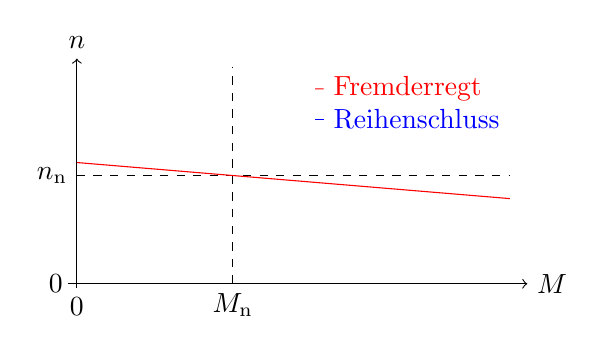
\begin{tikzpicture}[domain=0.9:10, samples=92, scale=0.55]
					\draw[->] (-0.2,0) -- (10.4,0) node[right] {$M$};
					\draw[->] (0,-0.1) -- (0,5.2) node[above] {$n$};
					\draw (0,-0.1) node[below] {$0$};
					\draw (-0.1,0) node[left] {$0$};
					\draw[blue, smooth] plot[id=Gleichstrommaschine1] function{ 1.5/ sqrt(0.1*x) };
					\draw[dashed] (0,2.5) -- (10,2.5);
					\draw[dashed] (3.6,0) -- (3.6,5);
					\draw (3.6,0) node[below] {$M_\mathrm{n}$};
					\draw (0,2.5) node[left] {$n_\mathrm{n}$};
					\draw[red] (0,2.8) -- (10,1.966666)  (5.5,4.5) -- (5.7,4.5) node[right]{Fremderregt};
					\draw[blue] (5.5,3.8) -- (5.7,3.8) node[right]{Reihenschluss};
				\end{tikzpicture}
			}{Kennlinien von Gleichstrommaschinen}
		}
	\end{columns}
	\speech{Reihenschlussmaschine}{1}{Bei der Reihenschlussmaschine sind Erreger- und Rotorkreis in Reihe miteinander verbunden. Der Erregerstrom ist daher gleich mit dem Ankerstrom. Diese Art von Motor wird häufig in einfachen Elektrogeräten an Wechselspannung eingesetzt und wird daher auch Universal Motor genannt. Als Gleichstrommaschine wurde sie früher vor allem in Traktionsantrieben zum Beispiel von Straßenbahnen eingesetzt. Heutzutage sind diese allerdings wegen des besseren Wirkungsgrades durch Drehstromantriebe mit Umrichter ersetzt.}
	\silence{2}\speech{Reihenschlussmaschine}{2}{Im Gegensatz zur fremderregten Gleichstrommaschine, deren Drehzahl-Drehmoment-kennlinie entsprechend der Gleichung eine Gerade ist, verhält sich die Reihenschlussmaschine nichtlinear. Ohne Belastung ist die Drehzahl theoretisch unendlich, die Maschine würde also so stark beschleunigen, bis sie sich selbst durch die Fliehkraft zerstört. Man sagt dazu: Die Maschine geht durch. Bei den Anwendungen als Traktionsantrieb kommt ein Leerlauf aber nie vor, das große Anlaufmoment ist hingegen gewünscht.}
	\silence{2}

\end{frame}
